%\usepackage{algorithm}
%\usepackage{algorithmic}

\chapter{多环结构构造}
多环即拥有不同数量顶点的环结构的多种组合。 

\section{环结构检测与提取}
环结构的提取过程可以分作两步:寻找组成环的特征点(分叉点和交叉点);根据特征点构造环结构。
\subsection{特征点检测}
我们用来组成环结构的特征点包括二值骨架化血管网络的分叉点和交叉点。在视网膜图像中,分叉点指的是一条血管由一条变为两条处的节点,通常为三叉点;交叉点指的是由于视网膜的两条血管发生覆盖、交叉,在图像上显示出相交的情况形成的点,通常为四叉点。 如图~\ref{34bifur}所示的三、四分叉点。
\begin{figure}[ht!]
  \centering
  \begin{minipage}[b]{0.45\linewidth} 
      \centering 
  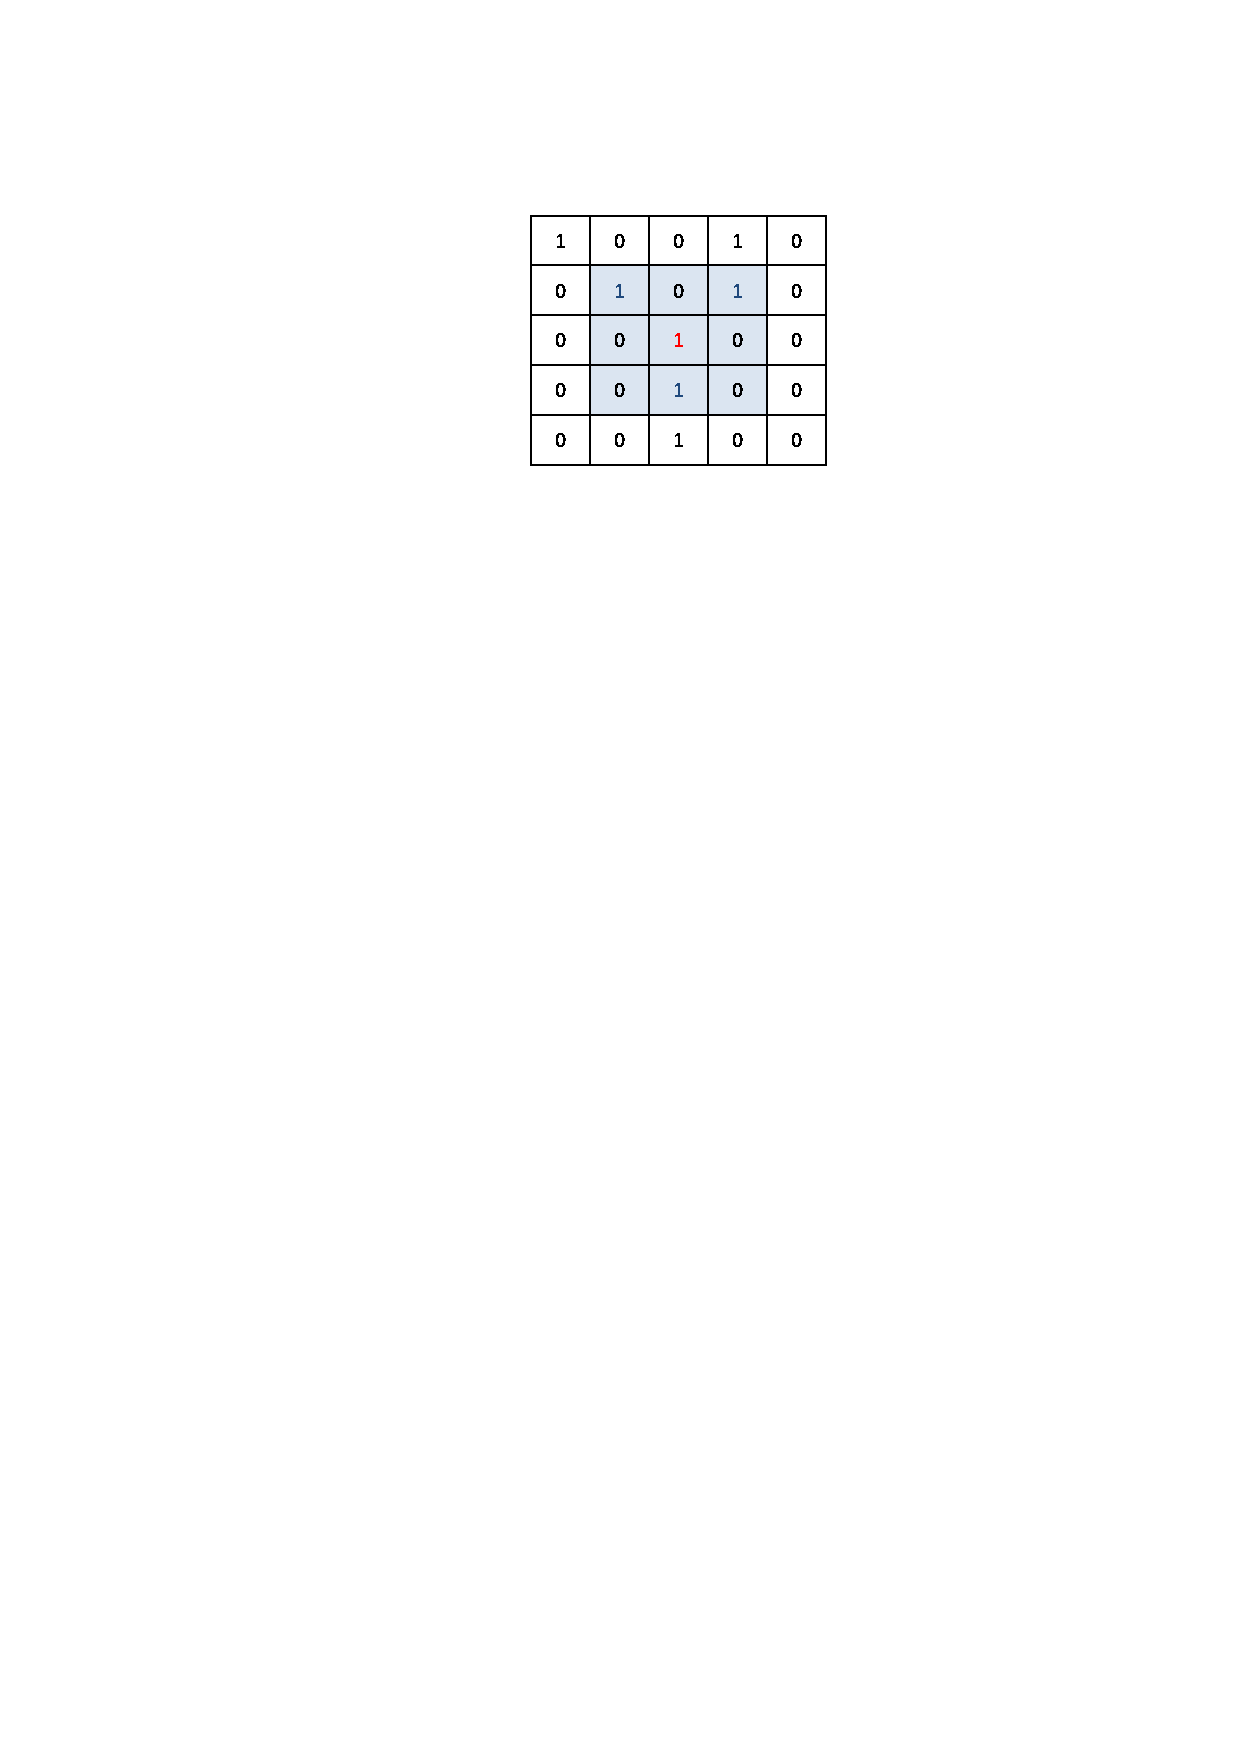
\includegraphics[width=0.9\linewidth]{3FeaturePoint.pdf}
        \centerline{(a)}\medskip
    \end{minipage}
  \begin{minipage}[b]{0.45\linewidth} 
      \centering 
  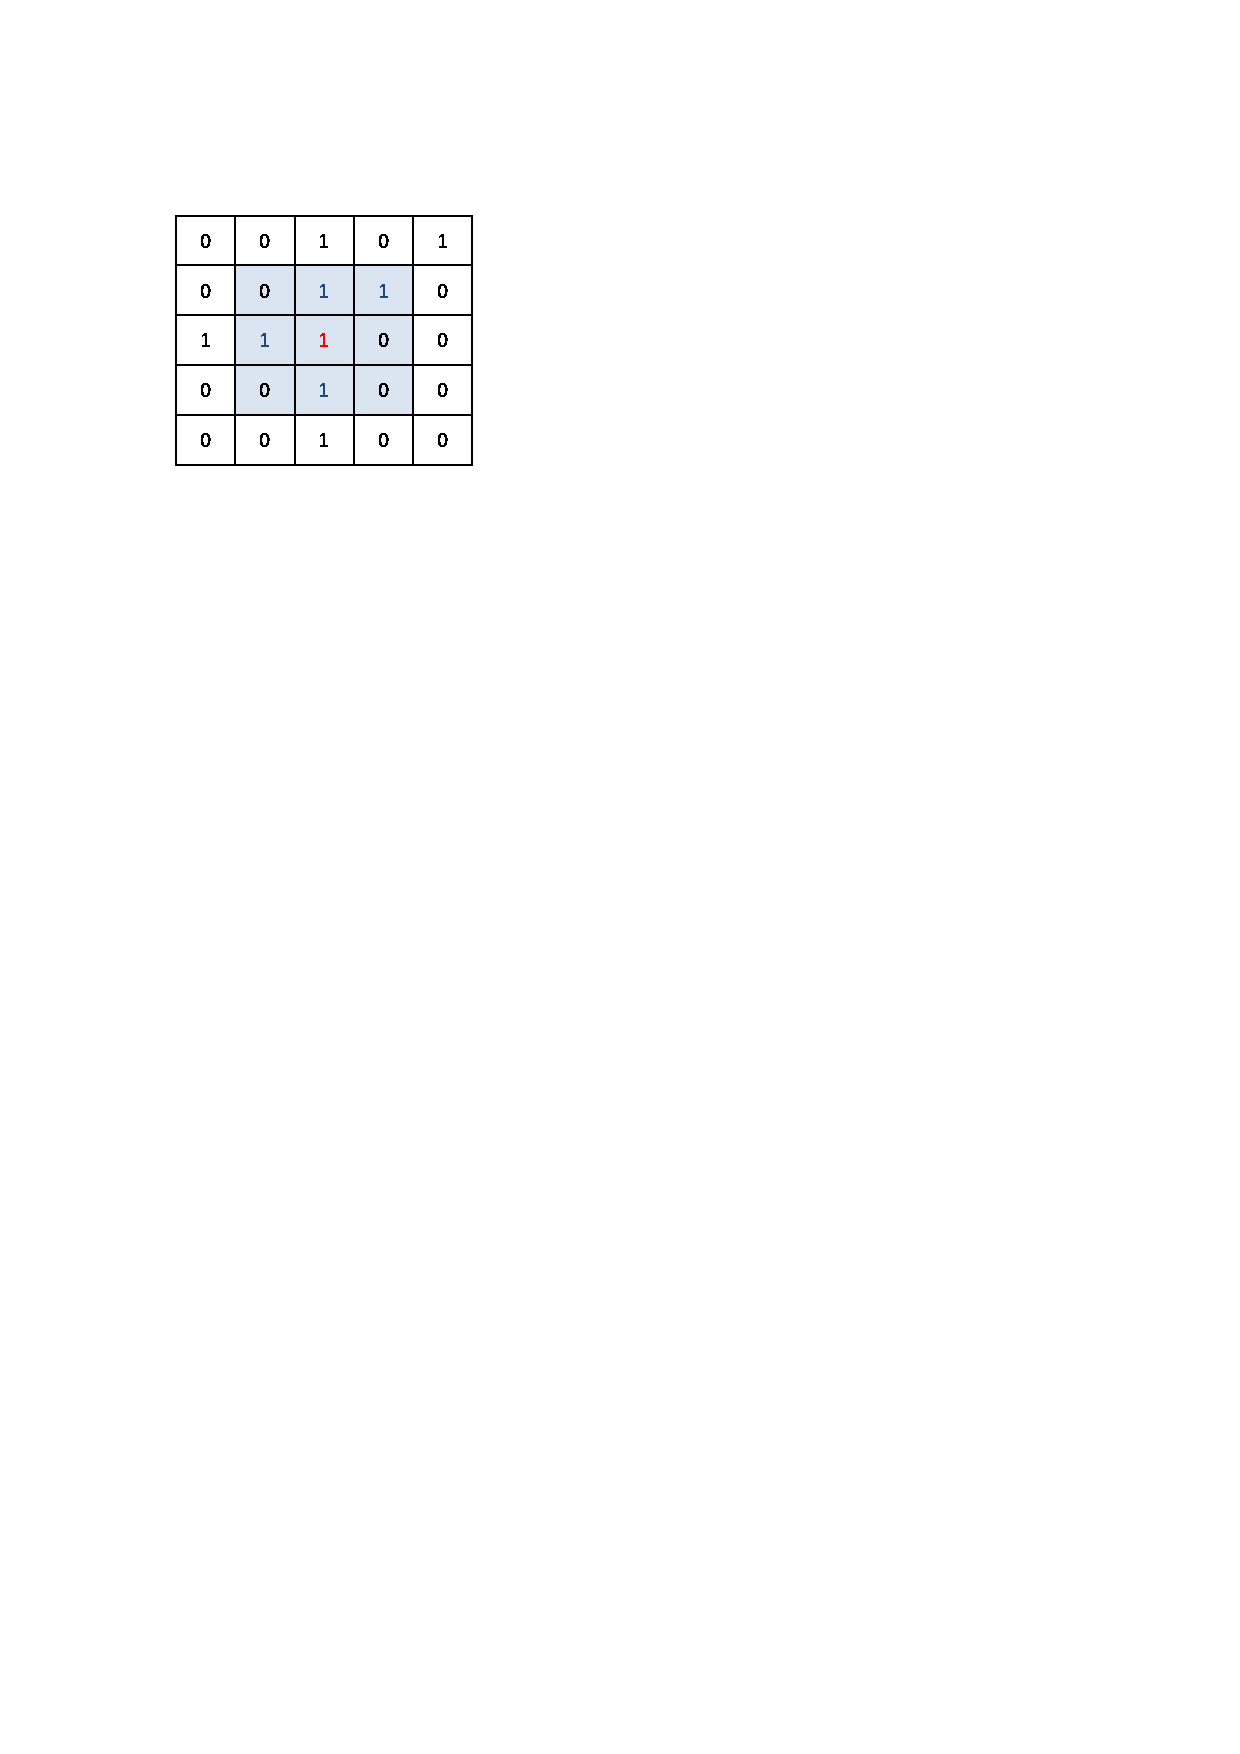
\includegraphics[width=0.9\linewidth]{4FeaturePoint.pdf}
    \centerline{(b)}\medskip
      \end{minipage}
  \caption{三叉点与四叉点}
    \label{34bifur}
 \end{figure}

特征点的搜索过程如下:

首先,已知在二值骨架化图像中,背景为黑,其像素值为0,血管骨架为白,其像素值为1。对图像中每个像素,计算其八邻域内像素值为1的个数,若像素值为1的个数大于等于3,则认为这个像素有可能为分叉点或交叉点,否则该像素只能是孤立点或血管上的普通一点。  

然后,将这些满足条件的点进行八连通区域标记(通过MATLAB的\emph{bwlabel}函数),构成该连通区域的每个点其八领域内像素值为1的个数都大于等于3,然后求得每个连通区域的一个或两个中心点。我们把这个中心点作为备选特征点,这主要考虑到三分叉点、四交叉点的特性及一些特殊的情况。其中,将所有连通区域按连通区域内的像素个数,分为简单连通区域(像素个数<6)和复杂连通区域(像素个数>=6)。构成简单连通区域的分叉点或交叉点一般较为标准,因此直接求取中心点即可,图~\ref{lian1}为简单连通区域的图例,红色处即为连通区域中心。
   \begin{figure}[ht!]
   \centering
  
\includegraphics[width=0.8\linewidth]{simple.png}
  \caption{简单连通区域图例}
    \label{lian1}
 \end{figure}
对于复杂连通区域,一般分为三种情况,一种是连通区域显示为两个分叉点或交叉点,而在实际图像中为一个分叉点,如图 ~\ref{lian2}所示,这种情况的处理方式与简单连通区域的处理方式相同;第二种是在该连通区域内存在多个分叉点或交叉点,首先要将它们合理区分开来,如图 ~\ref{lian3},图~\ref{lian4}所示为连通区域像素个数为6的情况,图 ~\ref{lian5}是连通区域像素个数大于6的情况。在这些情况下,需要先将它们分为两部分(两者分离方法略有不同),然后分别求出中心点,即为我们所求的备选特征点;第三种情况是由于骨架化处理不完全造成了连通区域内多像素聚集,分叉点或交叉点难以定位的问题,如图 ~\ref{lian6},图 ~\ref{lian7}所示,由于这种情况下的分叉点或交叉点定位不清晰,在后面的环结构匹配中无法和其他正常环结构进行比对,因此只简单求得该连通区域的中心点作为备选特征点即可。当处理复杂连通区域时,先判断是否为第一种情况,再依次处理下面的各种情况。
   \begin{figure}[ht!]
   \centering
  
\includegraphics[width=0.45\linewidth]{complex1}
  \caption{连通区域显示为两个分叉点,实际是一个分叉点的情况}
    \label{lian2}
 \end{figure}
    \begin{figure}[ht!]
   \centering
  
\includegraphics[width=0.45\linewidth]{complex5.png}
  \caption{连通区域像素个数为6的复杂情况之一}
    \label{lian3}
 \end{figure}
    \begin{figure}[ht!]
   \centering
  
\includegraphics[width=0.6\linewidth]{complex6.png}
  \caption{连通区域像素个数为6的复杂情况之二}
    \label{lian4}
 \end{figure}
    \begin{figure}[ht!]
   \centering
  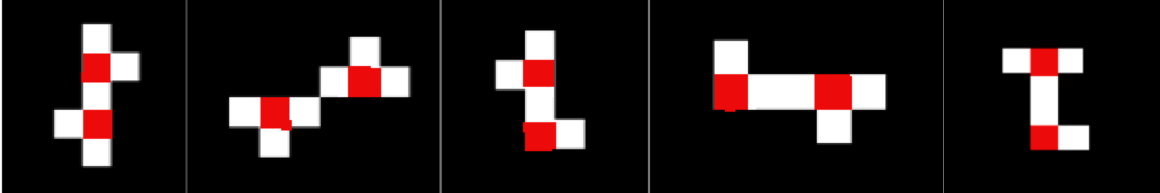
\includegraphics[width=0.6\linewidth]{complex_new.png}
  \caption{连通区域像素个数大于6的复杂情况}
    \label{lian5}
 \end{figure}
    \begin{figure}[ht!]
   \centering
  
\includegraphics[width=0.5\linewidth]{complex7.png}
  \caption{难以定位分叉点或交叉点的情况之一}
    \label{lian6}
 \end{figure}
    \begin{figure}[ht!]
   \centering
  
\includegraphics[width=0.45\linewidth]{complex3.png}
  \caption{难以定位分叉点或交叉点的情况之二}
    \label{lian7}
 \end{figure}

本文中求得中心点的方法主要采用了MATLAB的图像分析函数:\emph{regionprops}中的Centroid参数求重心。当该函数寻找到的中心处的像素其值为0(即没有实际像素点存在)时,则给该点赋值为1。这些特征点可以被看作图论中的顶点而与它们相连的血管可以被看作边。

找到特征点后,下一步需要求出各特征点之间的连接关系。具体方法如下:以一个特征点为起点,沿其八邻域逐渐向外搜索,当找到像素值为1的点时即判断该点是否为特征点,若该点为特征点则它即为与这个特征点相连的一个特征点,若不是特征点,说明该点为与这个特征点相连的血管上的一点,因此需要沿着该方向继续搜索。当所有方向全都搜索到特征点或已到血管末尾,则该特征点的搜索完成。此时另选一特征点重复上述步骤,直到所有特征点都找到与其相连的特征点,并将各特征点连接关系放入连接关系表中。

最后,我们采取了一种迭代去除无效特征点的方法对备选特征点进行筛选,即逐次去除度等于1的顶点(特征点),这是因为根据环的定义,一个顶点属于环当且仅当它有两个相邻的顶点。这样,经过这一步骤,就去除了一些独立的,不能构成环结构的特征点。

图 ~\ref{select}中的例子分别给出了备选特征点与经过滤除的最终的特征点。
 \begin{figure}[ht]
\centering
  \begin{minipage}[b]{0.48\linewidth} 
      \centering 
      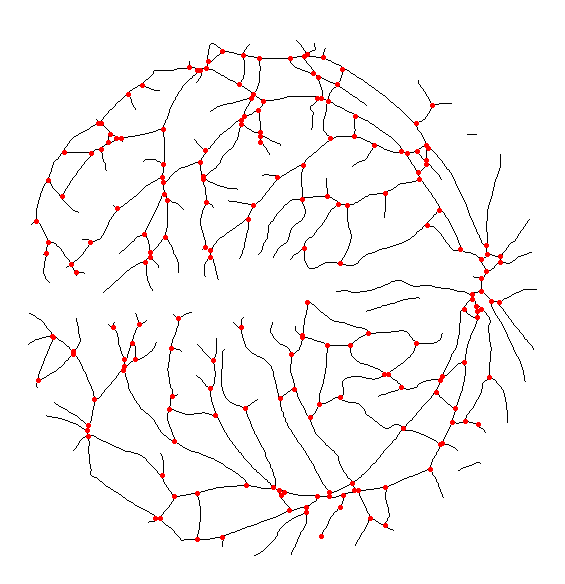
\includegraphics[width=0.9\linewidth]{36-select-before.png}
        \centerline{(a)}\medskip
    \end{minipage}
  \begin{minipage}[b]{0.48\linewidth}
    \centering
    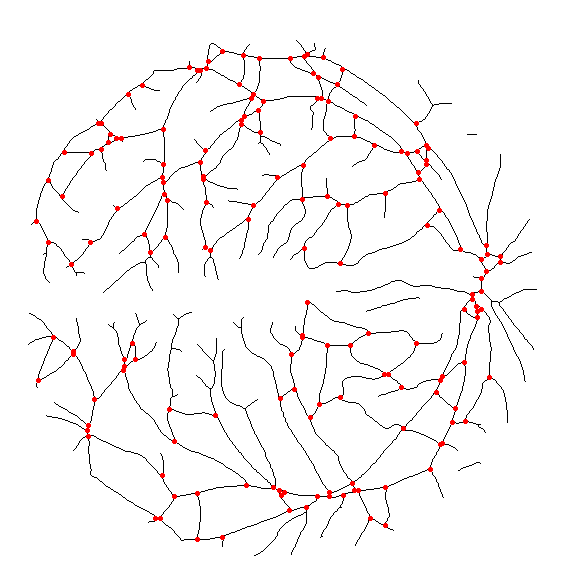
\includegraphics[width=0.9\linewidth]{36-select-after.png}
      \centerline{(b) }\medskip
  \end{minipage}
\caption{所有特征点及滤除后的特征点对比}
    \label{select}
\end{figure}


\subsection{基于SDFS的环结构提取算法}
正如上面提过的,从视网膜血管网络中寻找环结构等同于计算一个无向无权图的最小环基,而检测图中的最小环基现今是一个广泛讨论的问题,因此存在着多种计算最小环基的方法,这些方法通常涉及到图的遍历的知识。现今存在着两种遍历方法:深度优先搜索(DFS)与广度优先搜索(BFS),两种方法各有特点。

深度优先搜索的思想是:由一个初始点开始访问,继而访问这个点的一个邻接的顶点,若该邻接顶点未被访问过,从该顶点开始继续往深处搜索,直到当前顶点已被访问或已不存在邻接的顶点,然后回到原邻接点处继续搜索初始点的下一个邻接点,重复上述过程,一直到已发现从源顶点可达的所有顶点。广度优先搜索则是由初始点开始,访问一个顶点后,再访问它的邻接节点并且记录这个邻接节点,当访问完它的邻接节点之后就结束这个顶点的访问。然后进行下一层顶点的搜索,知道所有的顶点均被访问到,算法停止。图 ~\ref{dfs-bfs}为深度优先搜索与广度优先搜索的图示。
   \begin{figure}[ht!]
   \centering
  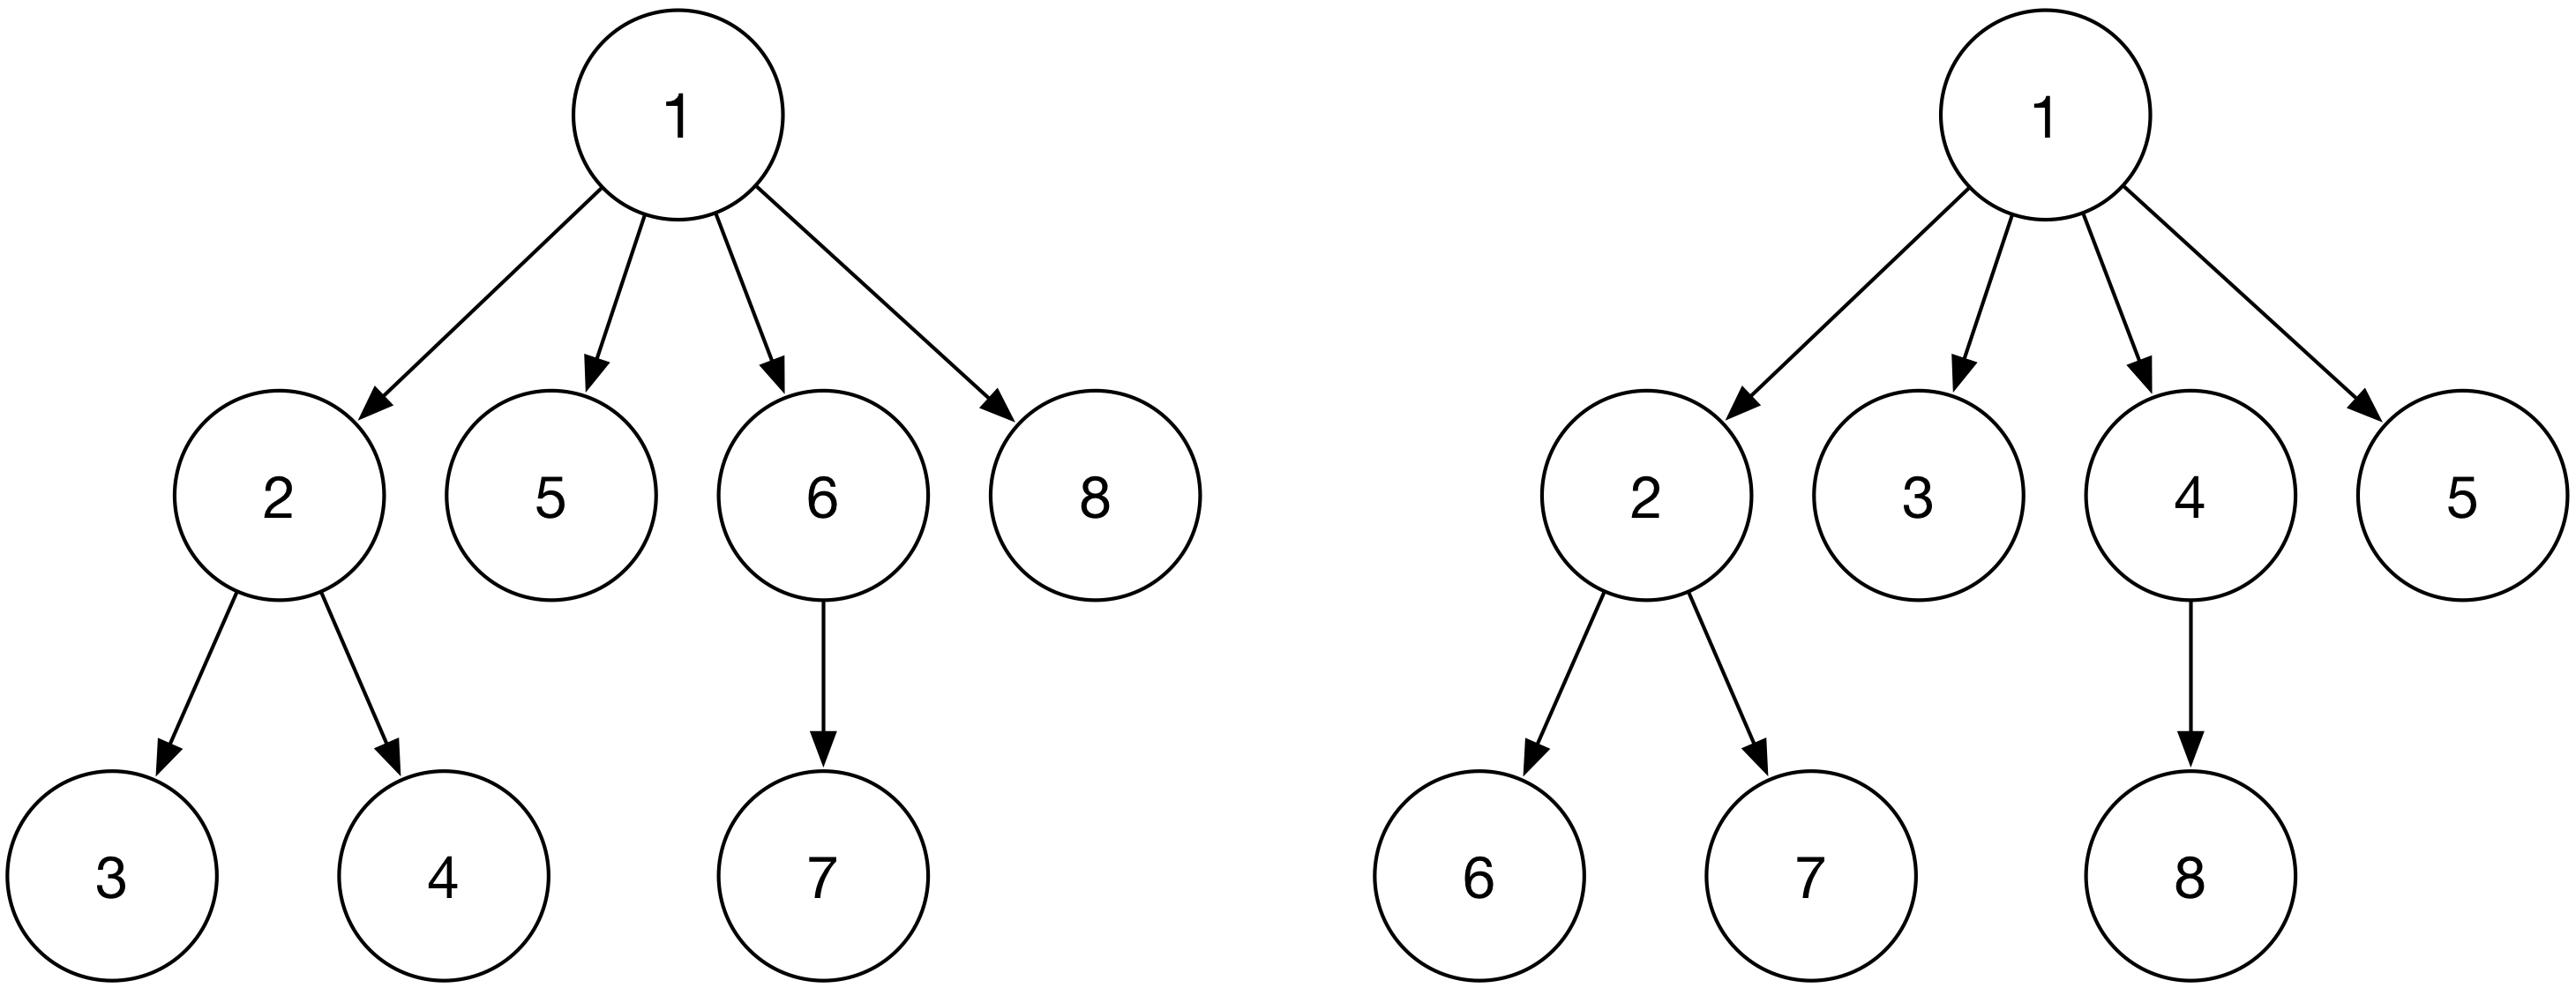
\includegraphics[width=0.8\linewidth]{dfs-bfs.png}
  \caption{深度优先搜索与广度优先搜索对比}
    \label{dfs-bfs}
 \end{figure}
 
我们观察到与普通的图相比,图像中的特征点存在固定的空间坐标而普通图的顶点通常不具有此种特点。因此我们通过结合特征点的空间坐标提出了基于空间的深度优先搜索算法(SDFS)来寻找环结构,算法过程如下,输入为特征点集与各特征点的连接关系:
\begin{enumerate}
\item 任取特征点集中的一点$a$为初始点。
\item 选择特征点集中任一且与初始点相连的特征点$b$,计算向量$V_{ba}$,将$a$、$b$按次序加入环结构路径中。 
\item 以点$b$为起点,找到所有与其相连的特征点$c_{i}(i=1,2,\cdots)$, 若特征点$c_i$在向量的顺时针的区域内,则将该点加入到右手区域点集中,若特征点在向量的逆时针的区域内,则将该点加入到左手区域点集中,如果特征点在向量上,则将该点加入到直线点集中。
\item 如果右手区域点集不为空,分别计算向量$V_{ba}$与向量$V_{bc_i}$的夹角,计算出其中最小的夹角,并将最小的夹角对应的特征点加入到环结构路径中。若右手区域点集为空而左手区域点集非空,以同样的方法求得使夹角最小的特征点加入到环结构路径中。若左手区域也为空,则将直线点集中的点加入到环结构路径中。
\item 判断新加入路径的点是否与环结构路径中第一个点相连且当前环结构路径中的点个数是否大于2,若相连则当前环结构路径中的所有点可能组成一个最小环,然后利用check函数检查该环是否真正是满足我们条件的环,若通过则输出该环,否则将$c_i$作为新的起点,重复步骤3-5,直到所有特征点的相邻关系已遍历完。
\item 以与$a$相连的其他点为起点,重复步骤2-5。
\item 选择除$a$外的其他点作为初始点,重复步骤1-6,直到所有特征点均遍历一遍。
\end{enumerate}

SDFS算法伪代码和check函数的伪代码分别如算法 ~\ref{algo1}、算法 ~\ref{algo2}所示。增加\emph{check}函数的目的是对环结构进行检查,因为在满足算法要求的前提下,还可能有如下~\ref{false_cycle}几种特殊情况,这些都不满足我们的最小环的概念,因此需要对该环结构路径进行检查。
   \begin{figure}[ht!]
   \centering
  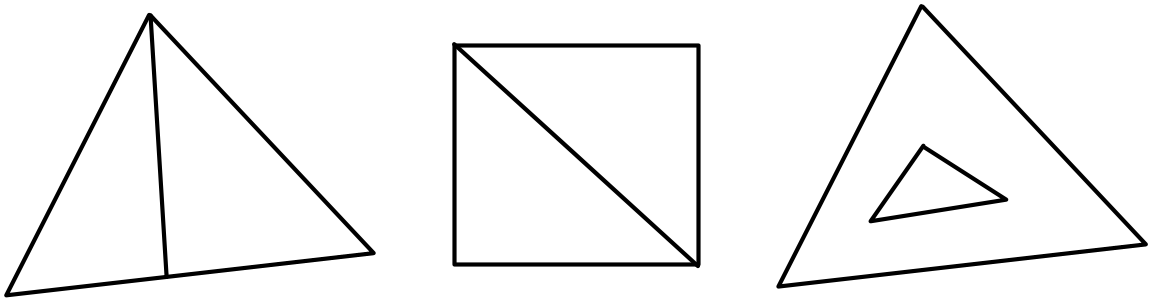
\includegraphics[width=0.8\linewidth]{checkcycle.png}
  \caption{不符合要求的环结构}
\label{false_cycle}
 \end{figure}


\begin{algorithm}[!ht]
\fontsize{12}{12}\selectfont{
\caption{\fontsize{12}{12}\selectfont{基于空间信息的深度优先搜索算法 (SDFS)}}
\label{algo1}
\textbf{Input}: 特征点集 $P$,二值骨架化图像中的特征点数量 $n$ 和连接关系矩阵 $M$。\\
\textbf{Output}: 骨架化二值图像中所有环结构,组成它们的特征点及连接关系。
\begin{algorithmic}[1]
\FOR {每个点 $a_i \in P$}
\FOR {每个点 $b_j\in P$ \AND 与 $a_i$相连}
\STATE 初始化路径 $CyclePath$ 
\STATE 将点 $a_i$ and $b_j$ 按顺序加入$CyclePath$ 
\WHILE {$n$$-$$-$}
\STATE $p_0\leftarrow CyclePath(end-1)$
\STATE $p_1\leftarrow CyclePath(end)$
\STATE 计算向量 $V_{p_1p_0}=V_{p_0}-V_{p_1}$
\FOR {每个点 $p_{2_k}\in P$ \AND 与 $p_1$相连}
\IF {$V_{p_1p_0}.x\times V_{p_1p_{2_k}}.y-V_{p_1p_0}.y\times V_{p_1p_{2_k}}.x>0$}
\STATE 添加 $p_{2_k}$ 到 $RightHandPoints$
\ELSIF {$V_{p_1p_0}.x\times V_{p_1p_{2_k}}.y-V_{p_1p_0}.y\times V_{p_1p_{2_k}}.x<0$}
\STATE 添加 $p_{2_k}$ 到 $LeftHandPoints$
\ELSE
\STATE 记录 $p_{2_k}$ 到$LinePoint$
\ENDIF
\ENDFOR
\IF {$RightHandPoints$ 非空}
\FOR {$RightHandPoints$中的每个点 $p_{2_m}$ }
\STATE 计算 $\theta_{p_0p_1p_{2_m}}=\arccos{\frac{V_{p_1p_0}\cdot V_{p_1p_{2_m}}}{\left|V_{p_1p_0}\right|\left|V_{p_1p_{2_m}}\right|}}$
\ENDFOR
\STATE   由 $\min{\left(\theta_{p_0p_1p_{2_m}}\right)}$选择对应的$p_{2_m}$加入到 $CyclePath$
\ELSIF {$LeftHandPoints$非空}
\FOR {$LeftHandPoints$中的每个点$p_{2_n}$}
\STATE 计算 $\theta_{p_0p_1p_{2_n}}=\arccos{\frac{V_{p_1p_0}\cdot V_{p_1p_{2_n}}}{\left|V_{p_1p_0}\right|\left|V_{p_1p_{2_n}}\right|}}$
\ENDFOR
\STATE 由 $\min{\left(\theta_{p_0p_1p_{2_n}}\right)}$ 选择对应的$p_{2_n}$加入到 $CyclePath$
\ELSE
\STATE 添加$LinePoint$到 $CyclePath$
\ENDIF
\IF  {$CyclePath$的特征点数大于$2$ \AND 最后一个特征点与第一个特征点相同}
\IF {$checkCyclePath(p_0,p_1,p_2,...)$}
\STATE 输出 $CyclePath(p_0,p_1,p_2,...) \Rightarrow Cycles$
\STATE break
\ENDIF
\ENDIF
\ENDWHILE
\ENDFOR  
\ENDFOR
\STATE 从 $Cycles$里去除重复的 $CyclePath$s
\end{algorithmic}
}
\end{algorithm}



\begin{algorithm}[!ht]
\fontsize{12}{12}\selectfont{
\caption{\fontsize{12}{12}\selectfont{环路径校验算法 checkCyclePath}}
\label{algo2}
\textbf{Input}: A $CyclePath$ 和特征点集  $P$. \\
\textbf{Output}: $True$ or $False$.
\begin{algorithmic}[1]
\FOR  {对每个点 $p_i\in P$ \AND $\notin CyclePath$}
\IF {$p_i$ 是由$CyclePath$组成的环上的边上的点 }
\RETURN $False$
\ELSIF {$p_i$是在由$CyclePath$组成的环结构区域内}
\RETURN $False$
\ENDIF
\ENDFOR
\FOR {每个点$c_{1_j}\in CyclePath$}
\FOR {每个点 $c_{2_k}\in CyclePath$ \AND 与 $c_{1_j}$不相邻}
\IF {$c_{1_j}$ 与 $c_{2_k}$相连}
\IF { $c_{1_j}c_{2_k}$的连接线在由 $CyclePath$组成的环区域内}
\RETURN $False$
\ENDIF 
\ENDIF 
\ENDFOR
\ENDFOR
\RETURN $True$
\end{algorithmic}
}
\end{algorithm}

我们提出的深度优先搜索算法可以有效利用图像的空间信息,不仅可以用来检测本文中的视网膜图像的环结构,还可以应用于其他基于图像的无向无权图的最小环基的搜索。通过计算,在一个有$n$个顶点的无向无权图中,本算法找到最小环基的时间复杂度为$O(n^2)$。

在本文中,考虑到视网膜血管的特性及后续配准算法复杂度,我们只采用三点环、四点环和五点环进行图像配准工作。

\section{环结构描述与匹配}
\subsection{环结构描述}
在参考图像和待配准图像中的所有环结构找到之后,需要对它们进行匹配,以决定用来进行变换及配准的环特征点。环结构是由动脉和静脉的血管的分叉点、交叉点及相连接的血管组成的结构,与其他特征相比,环结构更具唯一性,用来做配准的特征的可靠性更高,为了充分体现环结构的唯一性和可靠性,我们用环结构的分支长度、分支角度和相邻边的角度来描述一个环结构。图 ~\ref{descri}展示了一个四点环的描述例子。其中分支长度指的是两个特征点之间的像素距离,而分支角度需要依据以特征点为中心的分支血管上的邻域点来计算。
   \begin{figure}[ht!]
   \centering
  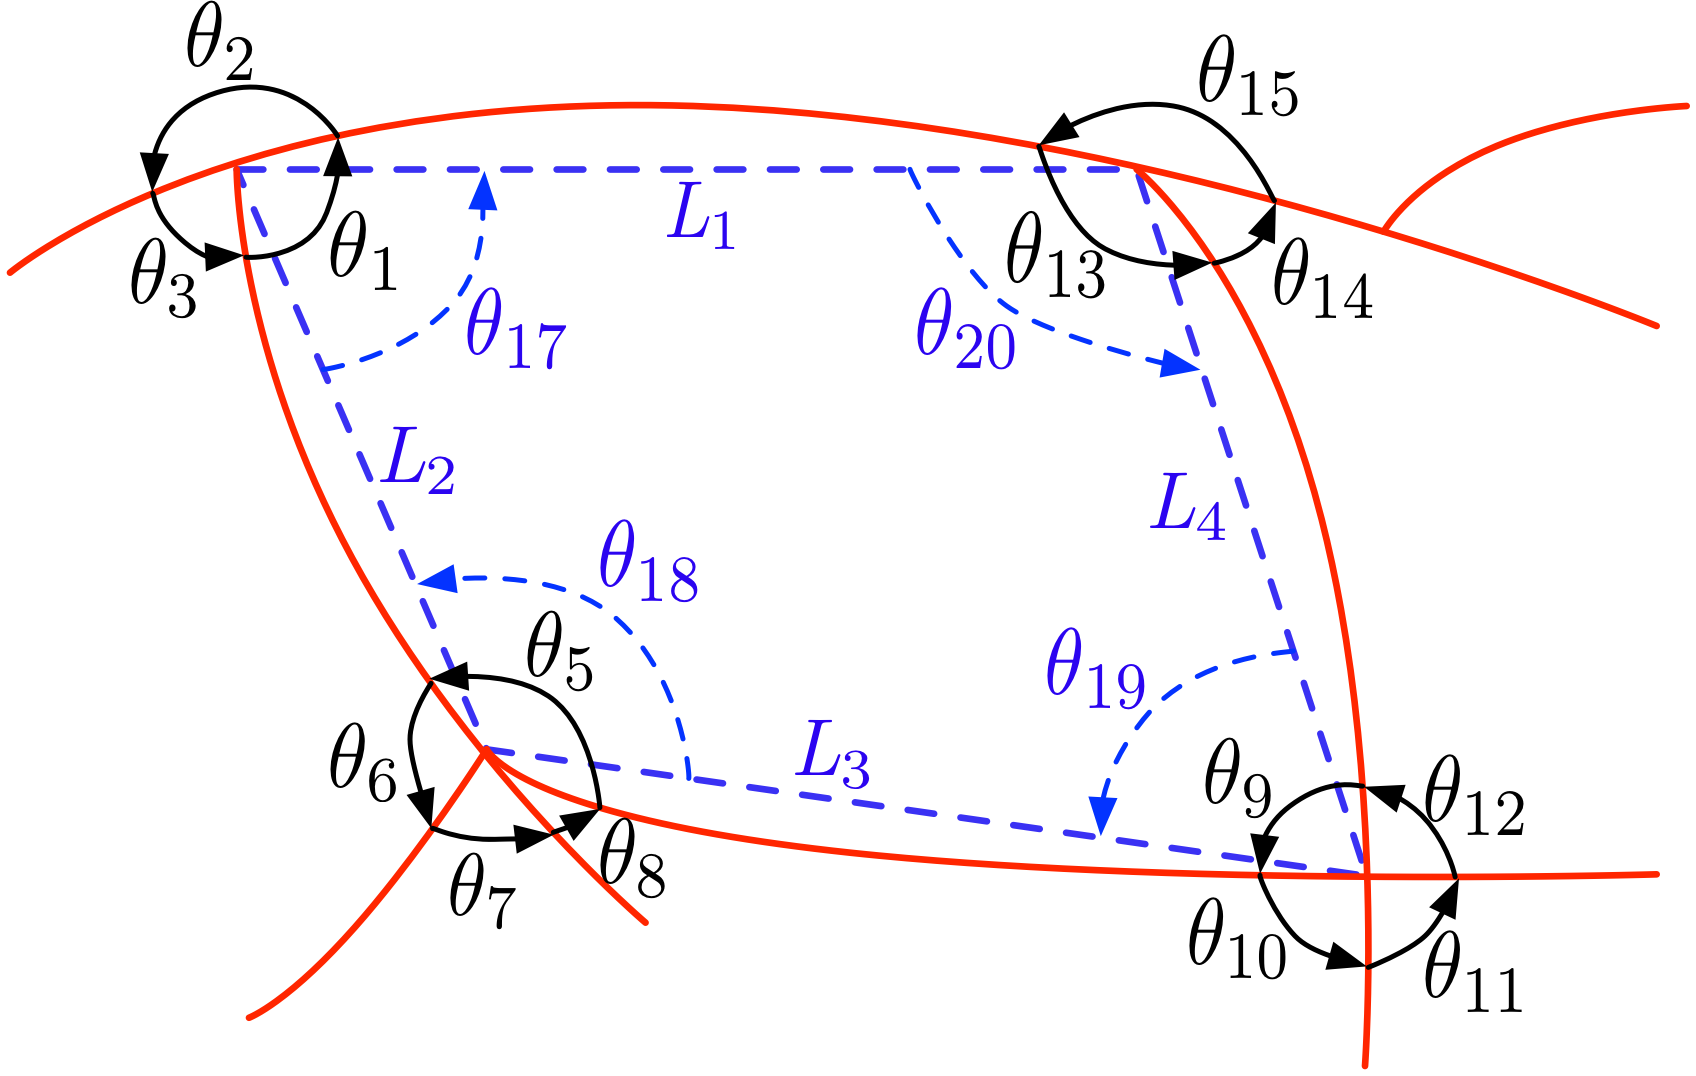
\includegraphics[width=0.6\linewidth]{description.png}
  \caption{环结构描述}
    \label{descri}
 \end{figure}

关于分支角度的计算过程如下,其中算法输入为二值图像$bw$,半径$R$:
\begin{enumerate}
\item 以分叉点(或交叉点)为中心,取$bw$ 一个$7\times7$(由$R$决定)的区域,以3点钟方向为起点,沿逆时针绕一圈求得连通区域最外围像素的值,见例图~\ref{bifur_ex}红色圈。
\item 以分叉点(或交叉点)为起点,$7\times7$ 区域的最外围点为终点,可以划分24 个方向的角度(如图~\ref{bifur_ex}蓝线所示)。
设分叉点为 $w(x_0,y_0)$, 24个邻域边缘像素坐标为$x_j,y_j,j=1,2,\ldots$,则分支方向为:
\begin{align}
\alpha_j = arctan\frac{dy}{dx}, dy = y_j - y_0, dx = x_j - x_0 
\end{align}	 	
由于反正切函数算出的范围为 $-90^{\circ} \sim 90^{\circ}$,需对求出的角度进行处理,以保证结果大于0:
\begin{align}
\beta_j = \left\{ \begin{array}{ll}
\alpha_j & \textrm{$dy \geq 0$, $dx \geq 0$} \\
\alpha_j + 180^{\circ} & \textrm{$dy \geq 0$, $dx \leq 0$ 或 $dy \leq 0$, $dx \geq 0$}\\
\alpha_j + 360^{\circ} & \textrm{$dy \leq 0, dx \leq 0$}
\end{array} \right.
\end{align}	 	
$\beta$即为24个方向的角度,注意每个角度并不是均为$15^{\circ}$。
\item 根据最外围值为1 的像素的位置,求得与3点钟方向对应的夹角;若遇到图~\ref{bifur_ex}中存在两个或多个值为1 的像素相邻的情况,取这两个像素和分叉点(或交叉点)中心连线与3点钟方向夹角的平均值作为此方向的角度值。
\item 夹角两两相减,若相减为负值则加上$360^{\circ}$,得到的角度$\theta$则为最终的分叉点(或交叉点)的角度(即图紫色处角度)。
\end{enumerate}
   \begin{figure}[ht!]
   \centering
  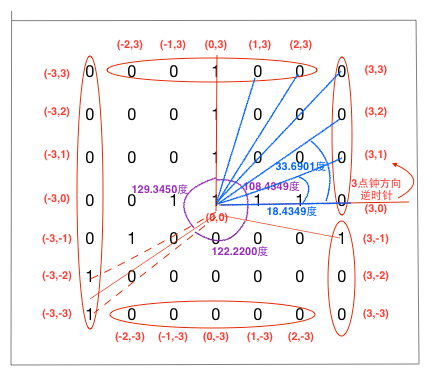
\includegraphics[width=0.7\linewidth]{分叉点图.png}
  \caption{特征点角度求解示意图}
    \label{bifur_ex}
 \end{figure}
上述环结构描述示例图 ~\ref{descri},$L_1\sim L_4$,$\theta_1\sim\theta_{16}$和$\theta_{17}\sim\theta_{20}$分别代表了一个四点环的分支长度,分支角度和邻域边之间的角度。
特征点之间的分支长度则为两者之间的欧氏距离:
\begin{align}
L = \sqrt{(y_j - y_0)^2 + (x_j - x_0)^2}, j = 1, 2, \ldots
\end{align}	 	
然后我们通过公式~\ref{length-angle}对所有边和角度进行归一化,归一化作为一种常见的数据处理手段,可以将数值的绝对值变成相对值的关系,通常是将需要处理的数据经过某种算法处理,限制在我们需要的一定范围内(如$(0,1)$),以确保各个归一化的参数能够相互比较,后面数据处理更加方便,在这里此项处理也是为了保证尺度不变性及旋转不变性。公式~\ref{vector2}给出了图~\ref{descri}例子中四点环最终的特征向量。
 \begin{equation}
 \begin{split}
L_{iNorm}&=\frac{L_i}{\sum{L}}\\
\theta_{jNorm}&=\frac{\theta_j}{360^\circ}
\end{split}
\label{length-angle}
\end{equation}	 	
 \begin{equation}
 \begin{split}
\tilde{v}=\{\textrm{长度,角度}\}=\{L_{1},L_{2},L_{3},L_{4},\theta_{1},\theta_{2},\theta_{3},\mathbf{0},\theta_{5},\\\theta_{6},\theta_{7},\theta_{8},\theta_{9},\theta_{10},\theta_{11},\theta_{12},\theta_{13},\theta_{14},\theta_{15},\mathbf{0},\theta_{17},\theta_{18},\theta_{19},\theta_{20}\}
\label{vector2}
 \end{split}
 \end{equation}
	 		 	
从上面求解特征向量过程可以看出,特征向量元素的个数是与环结构特征点数量有关的,而分支角度是与特征点的类型有关的,即分叉点通常是三分叉点而交叉点通常为四交叉点。为了得到同一长度的向量以用于后面的匹配,我们把所有环结构的特征点的分支角度按最大四个进行处理,因此三、四、五点环结构的特征向量变为18,24和30维,其中不存在的元素置为0,如公式~\ref{vector2}所示。

\subsection{相似性度量}
视网膜血管图像中,由三、四、五个分叉点(或交叉点)组成的环居多,同时考虑到后续环结构配准算法的复杂度,我们仅采用环结构检测算法得出的所有环中的三、四、五点环来作为配准特征。接下来,我们需要通过相似性度量完成参考图像与待配准图像中对应特征点数的环结构的匹配工作,以输出一一对应的三、四、五点环,用于下步的配准工作。其中相似性度量只在同种类型的环之间进行计算,得到最匹配的环结构。

基于特征的相似性度量,可以是依据于灰度值的,或者是依据对应特征之间的“距离”,这里的距离通常指的是根据对应特征结构的空间位置距离。这里我们采用的是“距离”方法。其中选择合适的距离函数十分重要,使用比较广泛的相似性度量、距离函数有范数和欧氏距离,曼哈顿距离,马氏距离,余弦相似度,汉明距离等。经过一定对比,这里我们采用曼哈顿距离作为相似性度量距离。

曼哈顿距离又称绝对值距离,在欧几里得空间中,为固定直角坐标系上两点所形成的线段的对轴产生的投影距离总和,它对应$L1$-范数。在$n$维空间中存在两个点$a(x_{11},x_{12},\ldots,x_{1n})$与$b(x_{21},x_{22},\ldots,x_{2n})$,它们间的曼哈顿距离定义如下:
\begin{equation}
d_{12}=\sum_{k=1}^n|x_{1k}-x_{2k}|
\end{equation}

对于二位平面上的两点$a(x_1,y_1)$与$b(x_2,y_2)$间的曼哈顿距离为:
\begin{equation}
d_{12}=|x_1-x_2|+|y_1-y_2|
\end{equation}
	 	
在视网膜图像中,对于参考图像中的$m$个环结构特征和待配准图像中的$n$个环结构特征,其曼哈顿距离相似性度量为:
\begin{align}
D_{pq} = mean(|V_p-W_q|), p = 1, 2, \ldots, m; q = 1, 2, \ldots, n
\end{align}	 	
其中$V_p$代表参考图像图像中的第$P$个环结构,$W_q$代表待配准图像中的第$q$个环结构,函数mean代表向量求均值运算。$D_{pq}$的值越小,表明两个环结构相似性越高。利用上述度量公式,同时为了保证当前环结构的特征点顺序正确,对参考图像与待配准图像的三、四、五点环分别进行循环移位匹配计算度量值,将结果按度量值从小到大排序,然后选择度量值最小的一组作为该环类型(三、四、五点环)做后续配准的环结构。
 
同时为了防止拥有最小相似性度量值的结果仍然是错误的,我们规定了一个阈值,若两图像的某种环结构的最小相似性度量值大于这个阈值,也认为它们是不匹配的,即该环类型不存在匹配的环结构。这样的话,参考和待配准视网膜图像最后用来配准的环结构中可能存在三、四、五点环空缺的情况,如流程图中所示的配准图像没有四点环结构。

\subsection{多环结构构造}
我们观察到,使用环结构进行配准的最后结果的准确性不取决于环结构的数量,而是取决于环结构特征的准确性,因此在参考图像与待配准图像存在多对满足条件的三、四、五点环结构时,我们只选择相似性度量值最小的一对(最优环)用作后续的配准。同时我们考虑到不同类型的最优环结构组合在一起,可能会产生不同的配准结果,因此在本文中提出了多环的概念,即将视网膜图像中最优的三点环、四点环和五点环相互组合作为配准特征,共产生七种组合(三点环、四点环、五点环、三四点环、三五点环、四五点环和三四五点环,如图~\ref{345}所示)。在配准时,同一组合中的环特征点一起作为变换过程的输入,进行配准。
   \begin{figure}[ht!]
   \centering
  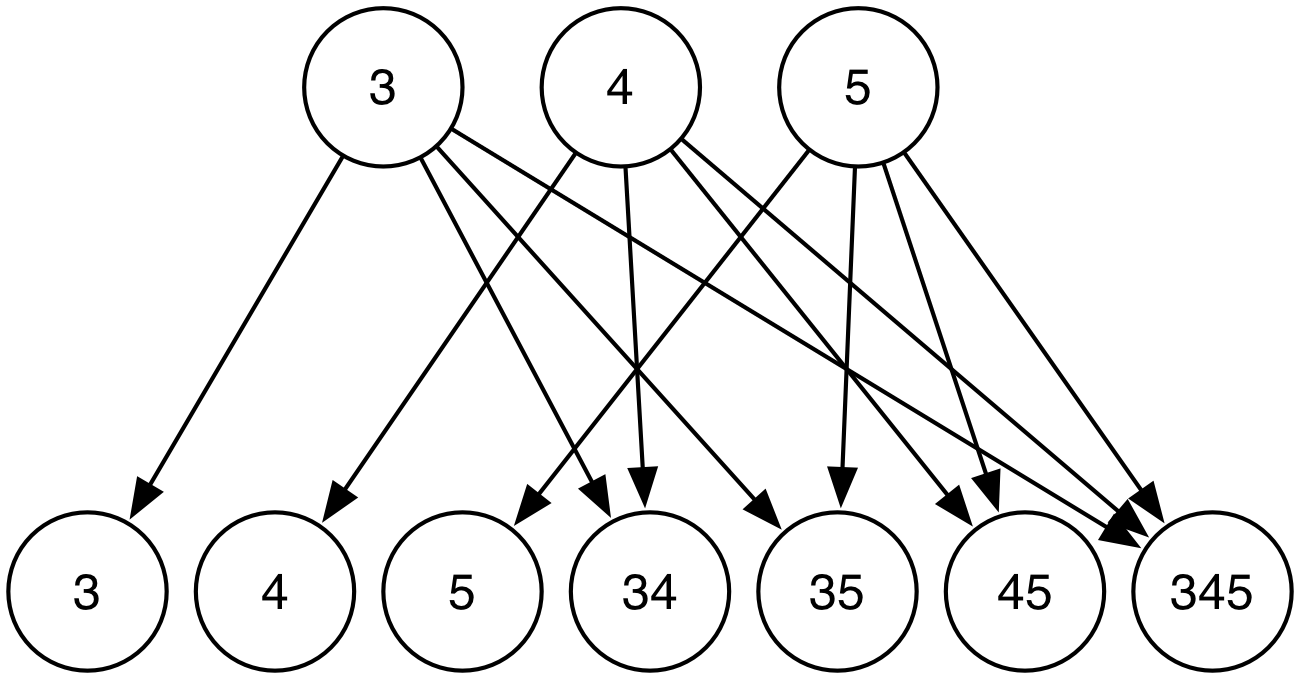
\includegraphics[width=0.7\linewidth]{345.png}
  \caption{7种环组合}
    \label{345}
 \end{figure}

\section{本章小结}
本章介绍了环结构检测的步骤:分叉点与交叉点检测、滤除无效特征点。阐述了一种新的环提取算法,不仅可以用来检测本文中的视网膜图像的环结构,还可以应用于其他基于图像的无向无权图的最小环基的搜索。同时,在考虑保证环结构唯一性和可靠性的基础上,提出了环结构描述方法,把环结构的特征表示为了特征向量。然后介绍了利用相似性度量以找到最优环结构的过程,并提出了多环结构的概念及构造方法,多环结构通过与预处理阶段的多尺度分割相结合,为下步的从局部到全局的配准工作奠定了基础。
